\documentclass{beamer}
\usepackage[utf8]{inputenc}
\usepackage{xcolor}
\usepackage{blindtext}
\renewcommand{\baselinestretch}{0.9}
\usepackage{url}
\usepackage{graphicx}
\usepackage{amsmath}
\usepackage{mathtools}
\graphicspath{{./images/}}
\usepackage{algorithm}  % http://ctan.org/pkg/algorithms
\usepackage{algcompatible}  % http://ctan.org/pkg/algorithmicx
\setbeamercovered{dynamic}
\usepackage{lipsum}  
\usepackage{hyperref}
\usepackage{colortbl}
\usetheme{Frankfurt}
\newtheorem{thm}{Pythagoras Theorem}

\title{Beamer Tutorial}
\subtitle{CS 213: SS Lab}

\author{Manav Kushwaha}
\institute[cse, IITDH]{Dep. of Comp. Sci. and Eng, IIT Dharwad}
\date{\today}
\logo{
\includegraphics[height=1cm]{../images/IITDH.jpg}}

\begin{document}
    
    \frame[plain]{\titlepage}
    
    \begin{frame}
    \frametitle{Table of Contents}
    \tableofcontents
    \end{frame}
    
    \section{Overlays}
    \subsection{Step-wise}
    \begin{frame}{$\backslash$pause}
        This is the first slide of this frame \\
        \pause{This is the 2nd slide of the this frame} \\
        \pause{These are created using \alert{$\backslash$pause} command} \\
        \pause{\alert{This is the 4th slide with alert}} \\
        \end{frame}
        
        \begin{frame}{$\backslash$item}
            \begin{enumerate}[<+->]
                \item This is first element of a list
                \begin{itemize}
                    \item But it might start to look silly
                    \item This has been done using the $\backslash$item of the list
                \end{itemize}
                \item So do remember
                \begin{description}
                    \item[Word 1] This is the definition of the word 1.
                    \item[Word 2] This is the definition of the word 2.
                \end{description}
            \end{enumerate}
        \end{frame}
    
    \begin{frame}[label=Test_label]{$\backslash$onslide}
        Default Text
        \begin{itemize}
            
            \item<2-> First Choice
            \item<3-> Second Choice
            \item<4-> Third Choice
        \end{itemize}
        \onslide<1-> Default onslide \\
        \onslide<2-> First onslide \\
        \onslide<3-> Second onslide \\
        \onslide<4-> Third onslide \\
    \end{frame}
    
    \subsection{Hiding Text}
    
    \begin{frame}{$\backslash$only}
    
        \only<1-2> {Only on the 1-2 slide\\}
        \only<3> {Only on the 3rd slide\\} 
        \only<2-4> {Only on 2-4 slides\\} 
        \only <3-4> {Only on 3-4 slides\\} 
        
    \end{frame}
    
    \begin{frame}{$\backslash$uncover}
        \uncover<1-2> {
            \begin{alertblock}{Testblock1}
                Sample Text 1
            \end{alertblock}
        }
        \uncover<2-> {
            \begin{alertblock}{Testblock2}
                Sample Text 2
            \end{alertblock}
        }
        \uncover<3-> {
            \begin{alertblock}{Testblock3}
                Sample Text 3
            \end{alertblock}
        }
        
    \end{frame}
    
    \subsection{Highliting Text}
    \begin{frame}{$\backslash$color}
        \color<1-2>{cyan}{Cyan color slide 1-2\\}
        \color<2-4>{orange}{Orange color from slide 2-4\\}
        \color<4>{blue}{Blue color from slide 4\\}
        \color<3->{red}{Red color from slide 3\\}
    \end{frame}

    \begin{frame}{$\backslash$alert}
        \alert{This is alert}   \pause \\
        This is a \alert{part} of sentence that is alert.
        
    \end{frame}
    
    \section{Hyperlinks}
    \begin{frame}{Hyperlinks}
        \url{www.google.com}
        \vfill
        \href{www.google.com}{This is a hypertext}
        \vfill
        \hyperlink{Test_label}{\beamergotobutton{Go to the Previous Frame}}
    \end{frame}
    
    \section{Structures}
    
    \subsection{Blocks}
    \begin{frame}{$\backslash$block}
    
        \begin{exampleblock}{Example-block title}
        This is the Example-Block Title
        \end{exampleblock}
        \pause
    
        \begin{block}{Block title}
        This is the Block Title
        \end{block}
        \pause
        
        \begin{alertblock}{Alert-block title}
        This is the Alert-Block Title
        \end{alertblock}
    \end{frame}
    
    \subsection{Columns}
    \begin{frame}{$\backslash$columns}
        \begin{columns}
            \begin{column}{0.3\textwidth}
                \begin{block}{Left column}
        			The Earth \\
        			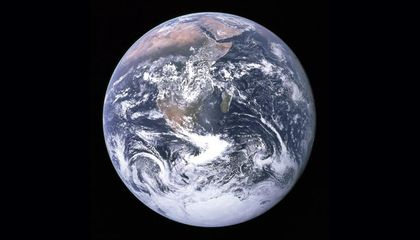
\includegraphics[width=1\textwidth]{images/Earth.jpg}
    		    \end{block}
                
            \end{column}
            \pause
            
            \begin{column}{0.3\textwidth}
                \begin{exampleblock}{Middle column}
        			Sample Text
    		    \end{exampleblock}
                
            \end{column}
            \pause
            
            \begin{column}{0.3\textwidth}
                \begin{alertblock}{Right column}
        			Sample Text 2
    		    \end{alertblock}
            \end{column}
        \end{columns}
    \end{frame}
    
    \section{Tables}
    \begin{frame}{ Tables Using $\backslash$pause }
        \begin{table}[h]
            \centering
            \caption{Test-Table}
            \begin{tabular}{p{2cm} |p{2cm} |p{2cm} |p{2cm} }
                \hline
                 1,1 & 1,2 & 1,3 & 1,4  \pause \\ 
                 2,1 & 2,2 & 2,3 & 2,4 \pause \\   
                 3,1 & 3,2 & 3,3 & 3,4 \pause \\
                 4,1 & 4,2 & 4,3 & 4,4  \\
                 \hline 
            \end{tabular}
            
            \label{tab:Test-Table1}
        \end{table}
    \end{frame}
    
    \begin{frame}{Tables using $\backslash$onslide}
    \centering
    \vfill
    \alert{Test Table 2 ( Column by Column)} \\
    \vfill
    \begin{tabular}{c<{\onslide<2->}c<{\onslide<3->}c<{\onslide<4->}c<{\onslide}c}
        \hline
         1,1 & 1,2 & 1,3 & 1,4  \\
         \hline
         2,1 & 2,2 & 2,3 & 2,4 \\
         3,1 & 3,2 & 3,3 & 3,4 \\
         4,1&4,2&4,3&4,4 \\
    \end{tabular}
\end{frame}
    
    \section{Transitions}
        \begin{frame}{$\backslash$transdissolve}
        \transdissolve
        \blindtext
        \end{frame}

        \begin{frame}{$\backslash$transboxout}
        \transboxout
        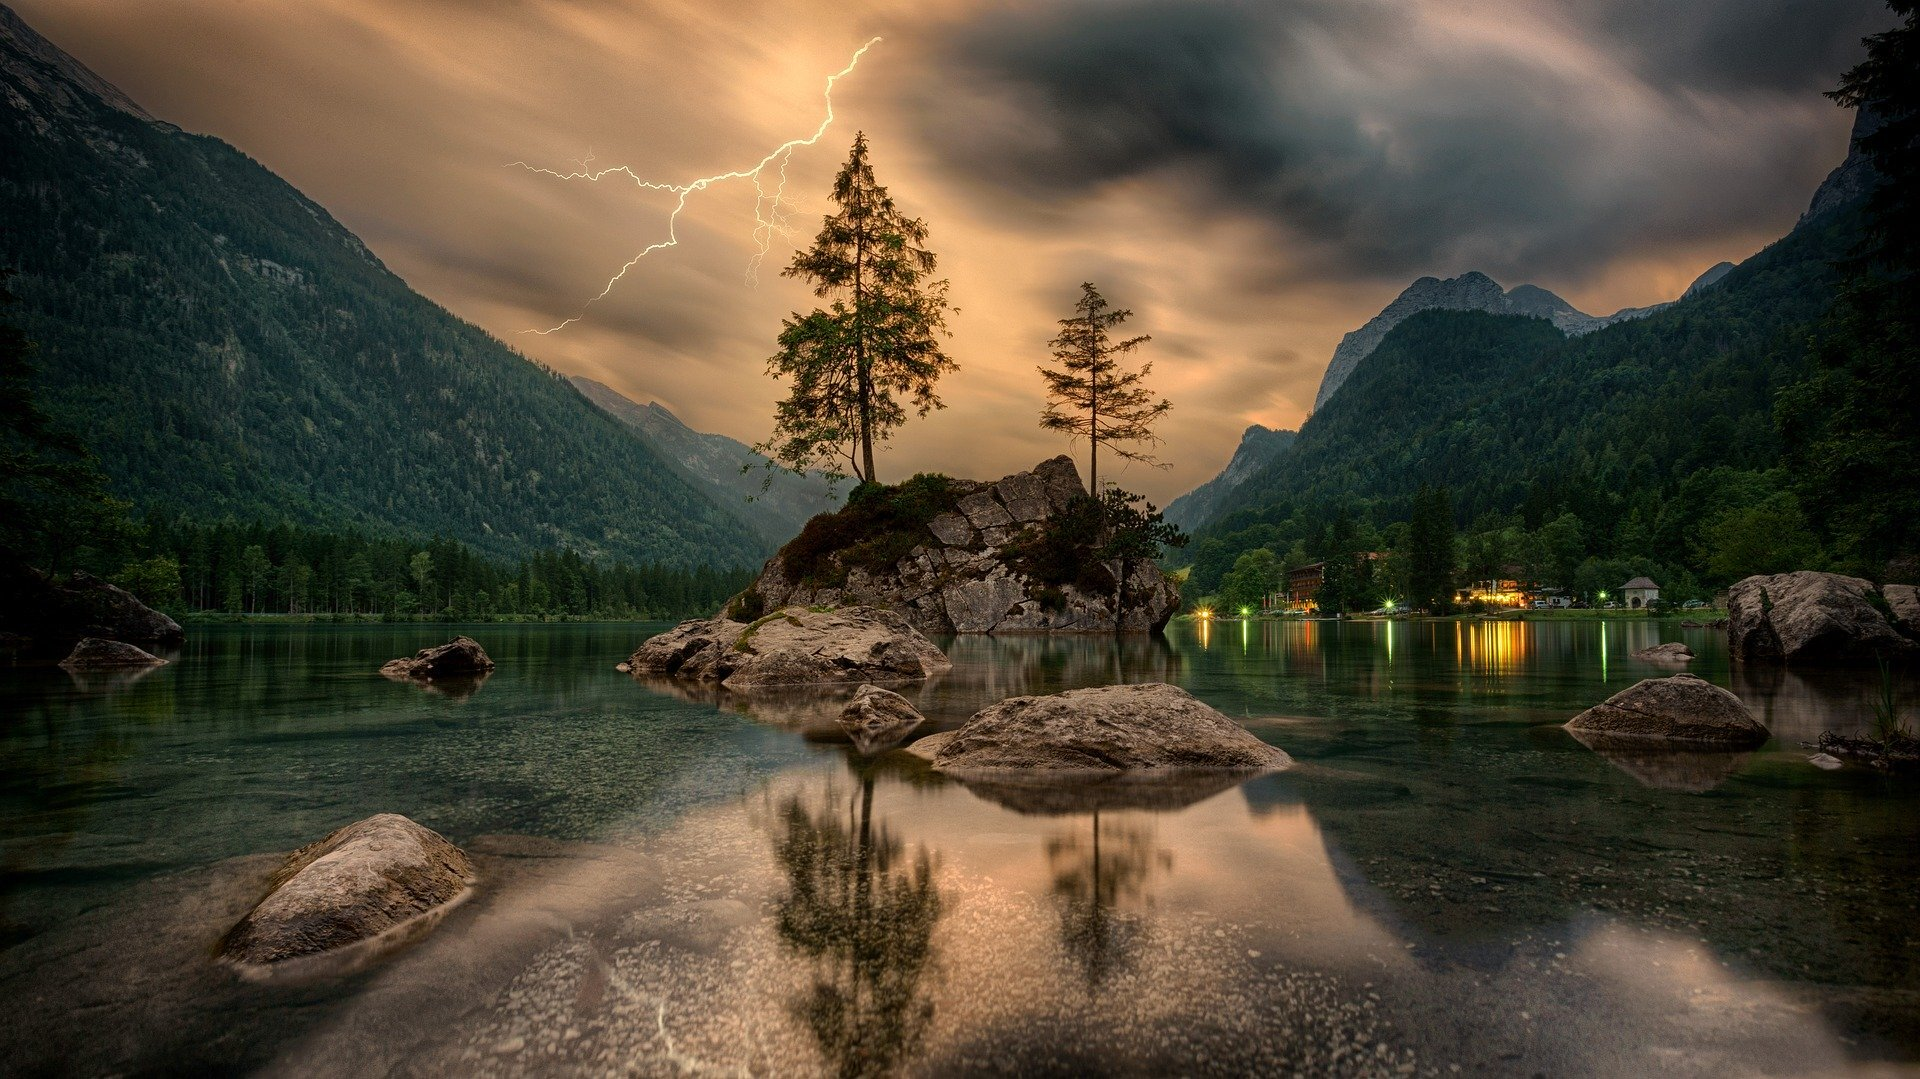
\includegraphics[width=0.7\textwidth]{images/nature1.jpg}
        \end{frame}
        
        \begin{frame}{$\backslash$transblindsvertical}
        \transblindsvertical
        \blindtext
        \end{frame}

        \section{Maths}
        \subsection{Algorithm}
        
        \begin{frame}[fragile]{An Algorithm For Printing Array in Reverse.}
        \begin{semiverbatim}
        \uncover<1->{\alert<0>{int main ()}}
        \uncover<1->{\alert<0>{\{}}
        \uncover<2->{\alert<2>{ \alert<4>{std::}vector<int> arr (100);}}
        \uncover<3->{\alert<3>{ for (int i = 0; i < 100; i++)}}
        \uncover<3->{\alert<2>{ \{}}
        \uncover<4->{\alert<4>{ \alert<2>{std::}cin>> arr[i]; }}
        \uncover<3->{\alert<3>{ \}}}
        \uncover<5->{\alert<5>{ for (int j = 99; j >= 0 ;j--)}}
        \uncover<6->{\alert<6>{ std::cout<<a[j]<<" ";}}

        \uncover<1->{\alert<0>{ return 0;}}
        \uncover<1->{\alert<0>{\}}}
        \end{semiverbatim}
        
        \end{frame}
        
        \subsection{Theorem}
        \begin{frame}{Theorem}
            \begin{thm}
                 The area of the square whose side is the hypotenuse (the side opposite the right angle) is equal to the sum of the areas of the squares on the other two sides.
            
            \begin{equation}
                a^2 + b^2 = c^2
            \end{equation} 
            \centering
            where c represents the length of the hypotenuse and a and b the lengths of the triangle's other two sides.
            \end{thm}
        \end{frame}
        
        \subsection{Multiline Equation}
        \begin{frame}{Multiline Equation}
            \begin{equation}
                \begin{aligned}
                    h = & \sqrt{(a+b)^2-4ab} \\ \pause
                      = & \sqrt{(a-b)^2} \\ \pause
                      = & |a-b|   
                \end{aligned}
            \end{equation}
        \end{frame}
        
        \section{Lists}
        
        \begin{frame}{$Lists$}
            The list of items are as follows:
                \begin{itemize}
                    \item <+-| alert@+> Some random text.
                    \item <+-| alert@+> Some random text 2.
                \end{itemize}
                
                \begin{enumerate}
                   \temporal<3> {}{ \item \alert{Hey Everyone}}{ \item Did anyone notice the alert on the previous slide} \pause
                    \item  Some random text.
                \end{enumerate}
                
                \begin{description}[<+->]
                   \uncover<5-> {\item[LOL]  Uncovered from slide 5.}
                   \uncover<6-> { \item[ROFL] Some random text again.}
                \end{description}
        \end{frame}
    
\end{document}